\chapter{Persistence Tools}

\section{Bracketing Algorithm}\label{bracketing}
This algorithm was implemented in Python for the experiments presented. 

\begin{algorithm}
\begin{algorithmic}
\Function{bracketing}{image, ANN, n, tol, n\_real, c\_i}
 \Comment{ start with same magnitude noise as image}
 \State u\_tol, l\_tol = 1.01, 0.99
 \State a\_var = Variance(image)/4 \Comment{Running Variance}
 \State l\_var, u\_var  = 0, a\_var*2\Comment{ Upper and Lower
   Variance of search space}
 \Comment{ Adversarial image plus noise counts}
 \State a\_counts = zeros(n)
 \State n\_sz = image.shape[0]
 \State mean = Zeros(n\_sz)
 \State I = Identity(n\_sz)
 \State count = 0
\Comment{grab the classification of the image under the network}
\State y\_a = argmax(ANN.forward(image))
\State samp = N(0, u\_var*I, n\_real)
\State image\_as = argmax(ANN.forward(image + samp))
\Comment{Expand search window}
\While{Sum(image\_as == y\_a) $>$ n\_real*tol/2}
\State u\_var = u\_var*2
\State samp = N(0, u\_var*I, n\_real)
\State image\_as = argmax(ANN.forward(image + samp))
\EndWhile
  \Comment{ perform the bracketing }
\For{i in range(0,n)}
\State count+=1
\Comment{compute sample and its torch tensor}
\State samp = N(0, a\_var*I, n\_real)

\State image\_as = argmax(ANN.forward(image + samp))

\State a\_counts[i] = Sum(image\_as == y\_a)

\Comment{floor and ceiling surround number}
\If{((a\_counts[i] $\leq$ Ceil(n\_real*(tol*u\_tol))) \& (a\_counts[i] $>$ Floor(n\_real*(tol*l\_tol))))}

        \Return{a\_var}
    \ElsIf{ (a\_counts[i] $<$ n\_real*tol)} \Comment{we're too high}
        \State u\_var = a\_var
        \State a\_var = (a\_var + l\_var)/2
    \ElsIf{ (a\_counts[i] $\geq$ n\_real*tol)} \Comment{we're too low}
        \State l\_var = a\_var
        \State a\_var = (u\_var + a\_var)/2
        \EndIf
\EndFor

   \Return{a\_var}
\EndFunction
\end{algorithmic}
\end{algorithm}

\begin{algorithm} [h!]
\begin{algorithmic}
\Function{bracketing}{image, classifier ($\CC$), numSamples, $\gamma$, maxSteps, precision}

\State $[\sigma_{\min},\sigma_{\max}] = $\textproc{rangefinder}(image, $\CC$, numSamples, $\gamma$)
\State count $=1$
\While{count$<$maxSteps}
\State $\sigma = \frac{\sigma_{\min}+\sigma_{\max}}{2}$
\State $\gamma_{\textnormal{new}} =$ \textproc{compute\_persistence}($\sigma$, image, numSamples, $\CC$)
\If{$|\gamma_{\textnormal{new}}-\gamma|<$precision}
\State \textbf{return} $\sigma$ %$\gamma_{\textnormal{new}}$
\ElsIf{$\gamma_{\textnormal{new}}>\gamma$}
\State $\sigma_{\min} = \sigma$
\Else
\State $\sigma_{\max} = \sigma$
\EndIf
\State count = count + 1
\EndWhile

\Return $\sigma$
\EndFunction

\\
\Function{rangefinder}{image, $\CC$, numSamples, $\gamma$}
\State $\sigma_{\min}=.5$,\;\; $\sigma_{\max}=1.5$
\State $\gamma_1 =$ \textproc{compute\_persistence}($\sigma_{\min}$, image, numSamples, $\CC$)
\State $\gamma_2 =$ \textproc{compute\_persistence}($\sigma_{\max}$, image, numSamples, $\CC$)
\While{$\gamma_1<\gamma$ \textbf{or} $\gamma_2>\gamma$}
\If{$\gamma_1<\gamma$}
\State $\sigma_{\min} = .5\sigma_{\min}$
\State $\gamma_1 =$ \textproc{compute\_persistence}($\sigma_{\min}$, image, numSamples, $\CC$)
\EndIf
\If{$\gamma_2>\gamma$}
\State $\sigma_{\max} = 2\sigma_{\max}$
\State $\gamma_2 =$ \textproc{compute\_persistence}($\sigma_{\max}$, image, numSamples, $\CC$)
\EndIf
\EndWhile

\Return{$[\sigma_{\min}, \sigma_{\max}]$}
%\sigma_{\min},\sigma_{\max}$}
\EndFunction

\\
\Function{compute\_persistence}{$\sigma$, image, numSamples, $\CC$}
\State sample = $N(\textnormal{image},\sigma^2I,$numSamples)
\State $\gamma_{\textnormal{est}} = \frac{|\{\CC(\textnormal{sample})=\CC(\textnormal{image})\}|}{\textnormal{numSamples}}$

\Return{$\gamma_{\textnormal{est}}$}
\EndFunction
\end{algorithmic}
\caption{Bracketing algorithm for computing $\gamma$-persistence}\label{bracketing}
\end{algorithm}


\section{Bracketing Algorithm}\label{sec:bracketing}
The Bracketing Algorithm is a way to determine persistance of an image with respect to a given classifier, typically a DNN. The algorithm was implemented in Python for the experiments presented. The \textproc{rangefinder} function is not strictly necessary, in that one could directly specify values of $\sigma_{\min}$ and $\sigma_{\max}$, but we include it here so that the code could be automated by a user if so desired.  

% \begin{algorithm} [h!]
% \begin{algorithmic}
% \Function{bracketing}{image, DNN, numSamples, $\gamma$, maxSteps, precision}
%  \Comment{ start with same magnitude noise as image}
%  \State u\_tol, l\_tol = 1+ precision, 1-precision
%  \State a\_var = Variance(image)/4 \Comment{Running Variance}
%  \State l\_var, u\_var  = 0, a\_var*2\Comment{ Upper and Lower
%   Variance of search space}
%  \Comment{ Adversarial image plus noise counts}
%  \State a\_counts = zeros(n)
%  \State n\_sz = image.shape[0]
%  \State mean = Zeros(n\_sz)
%  \State I = Identity(n\_sz)
%  \State count = 0
% \Comment{grab the classification of the image under the network}
% \State y\_a = argmax(DNN.forward(image))
% \State samp = N(0, u\_var*I, numSamples)
% \State image\_as = argmax(DNN.forward(image + samp))
% \Comment{Expand search window}
% \While{Sum(image\_as == y\_a) $>$ numSamples*$\gamma$/2} \Comment{Gaussian sampling}
% \State u\_var = u\_var*2
% \State samp = N(0, u\_var*I, numSamples)
% \State image\_as = argmax(DNN.forward(image + samp))
% \EndWhile
%   \Comment{ perform the bracketing }
% \For{i in range(1,maxSteps)}
% \State count+=1
% \Comment{compute sample and its torch tensor}
% \State samp = N(0, a\_var*I, numSamples)

% \State image\_as = argmax(DNN.forward(image + samp))

% \State a\_counts[i] = Sum(image\_as == y\_a)

% \Comment{floor and ceiling surround number}
% \If{((a\_counts[i] $\leq$ Ceil(numSamples*($\gamma$*u\_tol))) \& (a\_counts[i] $>$ Floor(numSamples*($\gamma$*l\_tol))))}

%         \Return{a\_var}
%     \ElsIf{ (a\_counts[i] $<$ numSamples*$\gamma$)} \Comment{we're too high}
%         \State u\_var = a\_var
%         \State a\_var = (a\_var + l\_var)/2
%     \ElsIf{ (a\_counts[i] $\geq$ numSamples*$\gamma$)} \Comment{we're too low}
%         \State l\_var = a\_var
%         \State a\_var = (u\_var + a\_var)/2
%         \EndIf
% \EndFor

%   \Return{a\_var}
% \EndFunction
% \end{algorithmic}
% \caption{Bracketing algorithm for computing $\gamma$-persistence}\label{bracketing}
% \end{algorithm}


\section{Convolutional neural networks used} \label{appendix:CNNs}
In Table \ref{table1} we reported results on varying complexity convolutional neural networks. These networks consist of a composition of convolutional layers followed by a maxpool and fully connected layers. 
The details of the network layers are described in Table \ref{tab:CNN} where Ch is the number of channels in the convolutional components. %\todo{[DG]: We need to simplify to the tables without the truncation}

%\vspace{.4cm}
\begin{table}[pt]
\centering
\caption{Structure of the CNNs C-Ch used in Table \ref{table1}}
\label{tab:CNN}
\begin{tabular}{llllll}
\toprule
     Layer & Type & Channels & Kernel & Stride & Output Shape \\
\midrule
     0 & Image & 1 & NA & NA & $(1, 28, 28)$ \\
     1 & Conv & Ch & $(5,5)$& $(1,1)$& $(\textnormal{Ch}, 24, 24)$\\
     2 & Conv & Ch & $(5,5)$& $(1,1)$& $(\textnormal{Ch}, 20, 20)$\\
     3 & Conv & Ch & $(5,5)$& $(1,1)$& $(\textnormal{Ch}, 16, 16)$\\
     4 & Conv & Ch & $(5,5)$& $(1,1)$& $(\textnormal{Ch}, 12, 12)$\\
     5 & Max Pool & Ch & $(2, 2)$ & $(2, 2)$& $(\textnormal{Ch}, 6, 6)$ \\
     %6 & Trunc & 1 & NA & NA & $Ch$ \\
     7 & FC & $(\textnormal{Ch}\cdot 6 \cdot 6, 256)$ & NA & NA & 256 \\
     8 & FC & $(256, 10)$ & NA & NA & 10 \\
     \bottomrule
\end{tabular}
\end{table}
 
%[DG: What changes if the number of channels changes? Can we give a general form.]
%We denote such a network as ``C-Ch-$k$,'' where C reflects that this is a convolutional DNN, Ch denotes the number of channels and $k$ denotes the width of the smallest level, for instance, ``C-128-2''.

\section{Additional Figures}
In this section we provide additional figures to demonstrate some of the experiments from the paper.

%\subsection{Figures interpolating between natural and adversarial examples}
%In this section we further investigate what happens on the straight line from a natural example to an adversarial example.

\subsection{Additional figures from MNIST}
In Figure \ref{fig:mnistadv} we begin with an image of a \texttt{1} and generate adversarial examples to the networks described in Section \ref{sec:mnist} via IGSM targeted at each class \texttt{2} through \texttt{9}; plotted are the counts of output classifications by the DNN from samples from Gaussian distributions with increasing standard deviation; this complements Figure \ref{fgsmo} in the main text. Note that the prevalence of the adversarial class falls off quickly in all cases, though the rate is different for different choices of target class.
\begin{figure}[!htb]
    \centering
    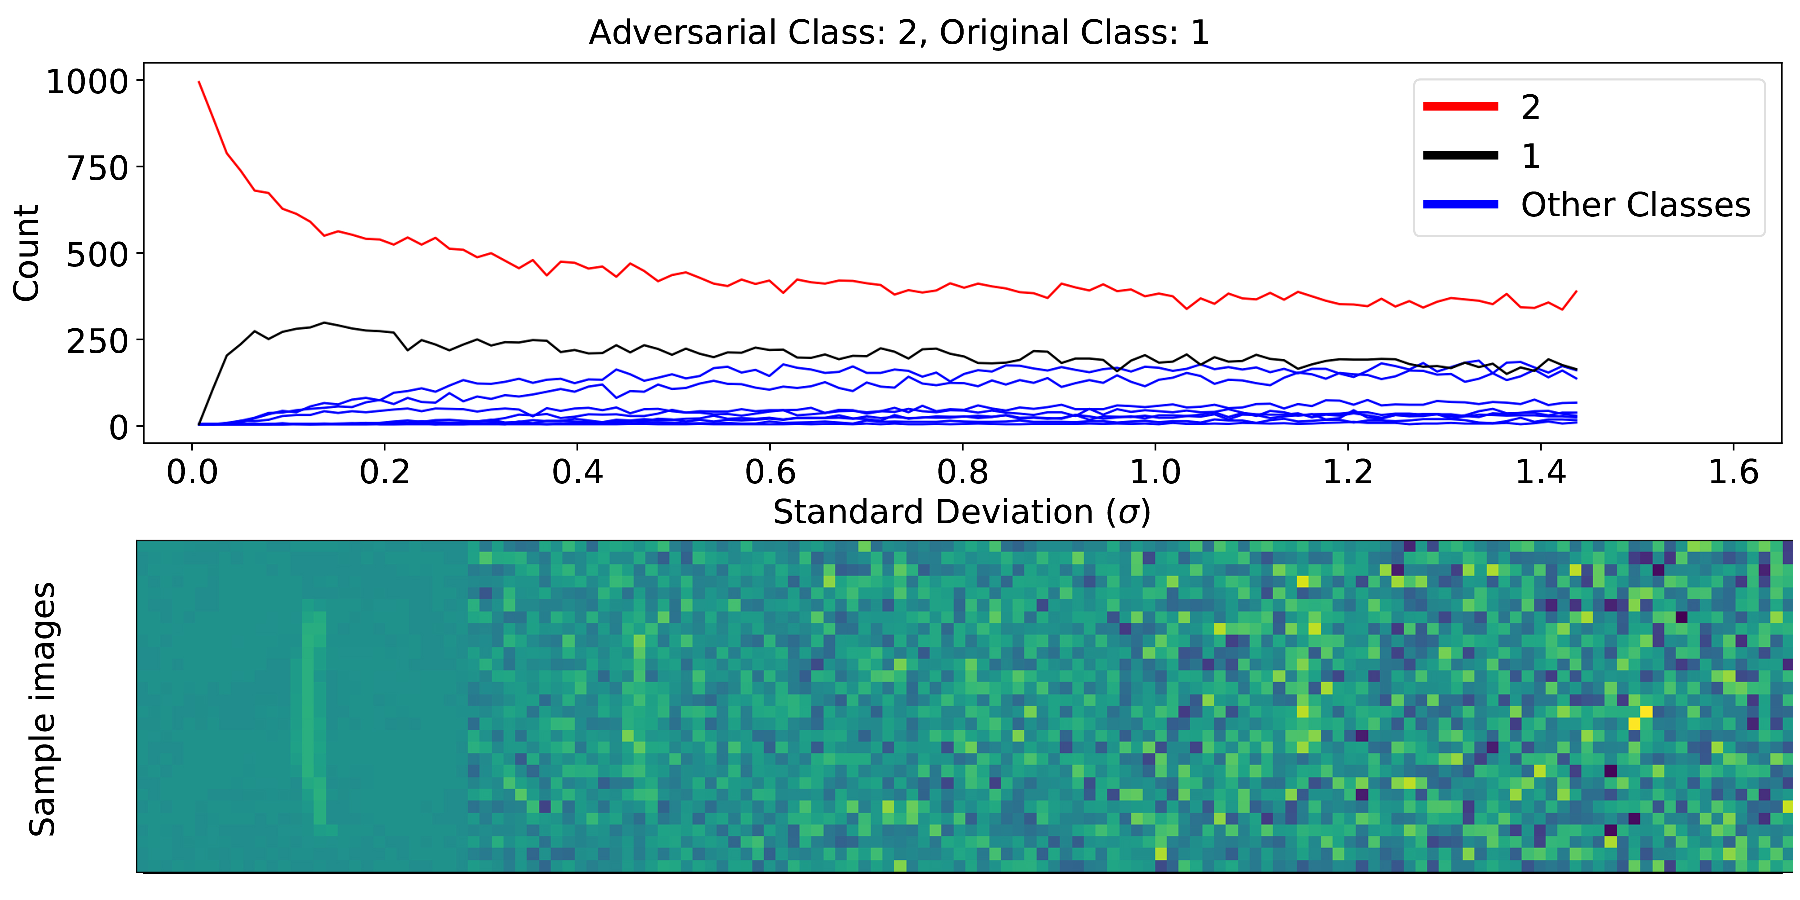
\includegraphics[width=.49\textwidth]{c2_figures/MNISTA2O1.pdf}
    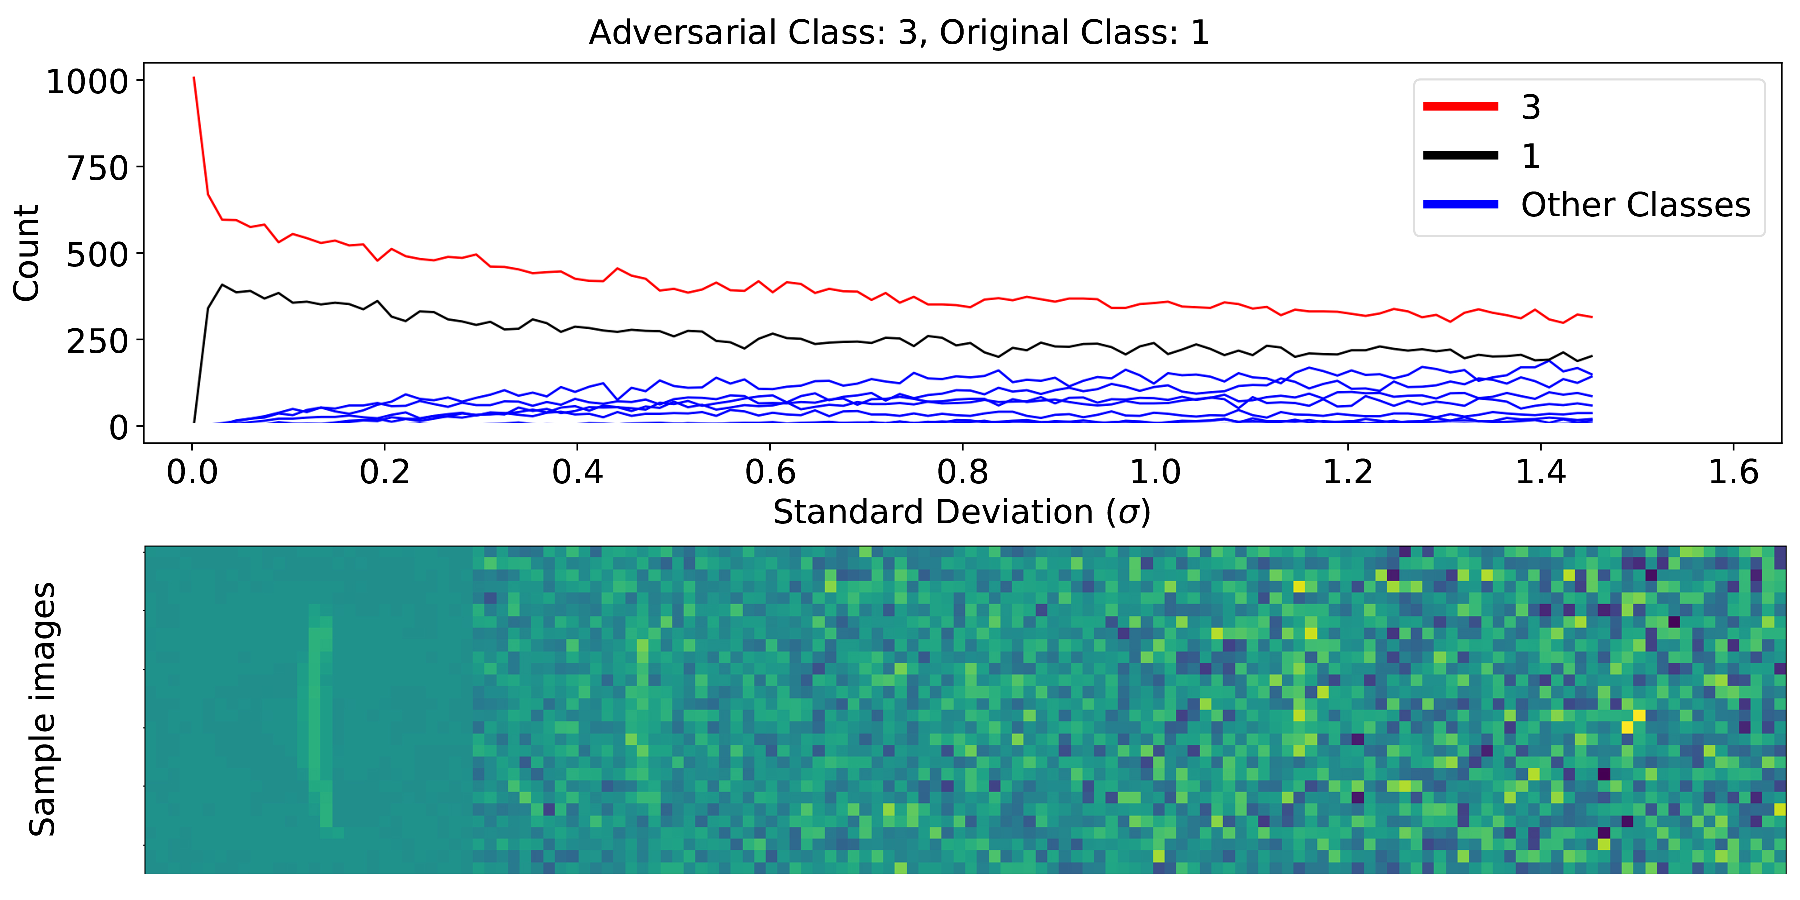
\includegraphics[width=.49\textwidth]{c2_figures/MNISTA3O1.pdf}
    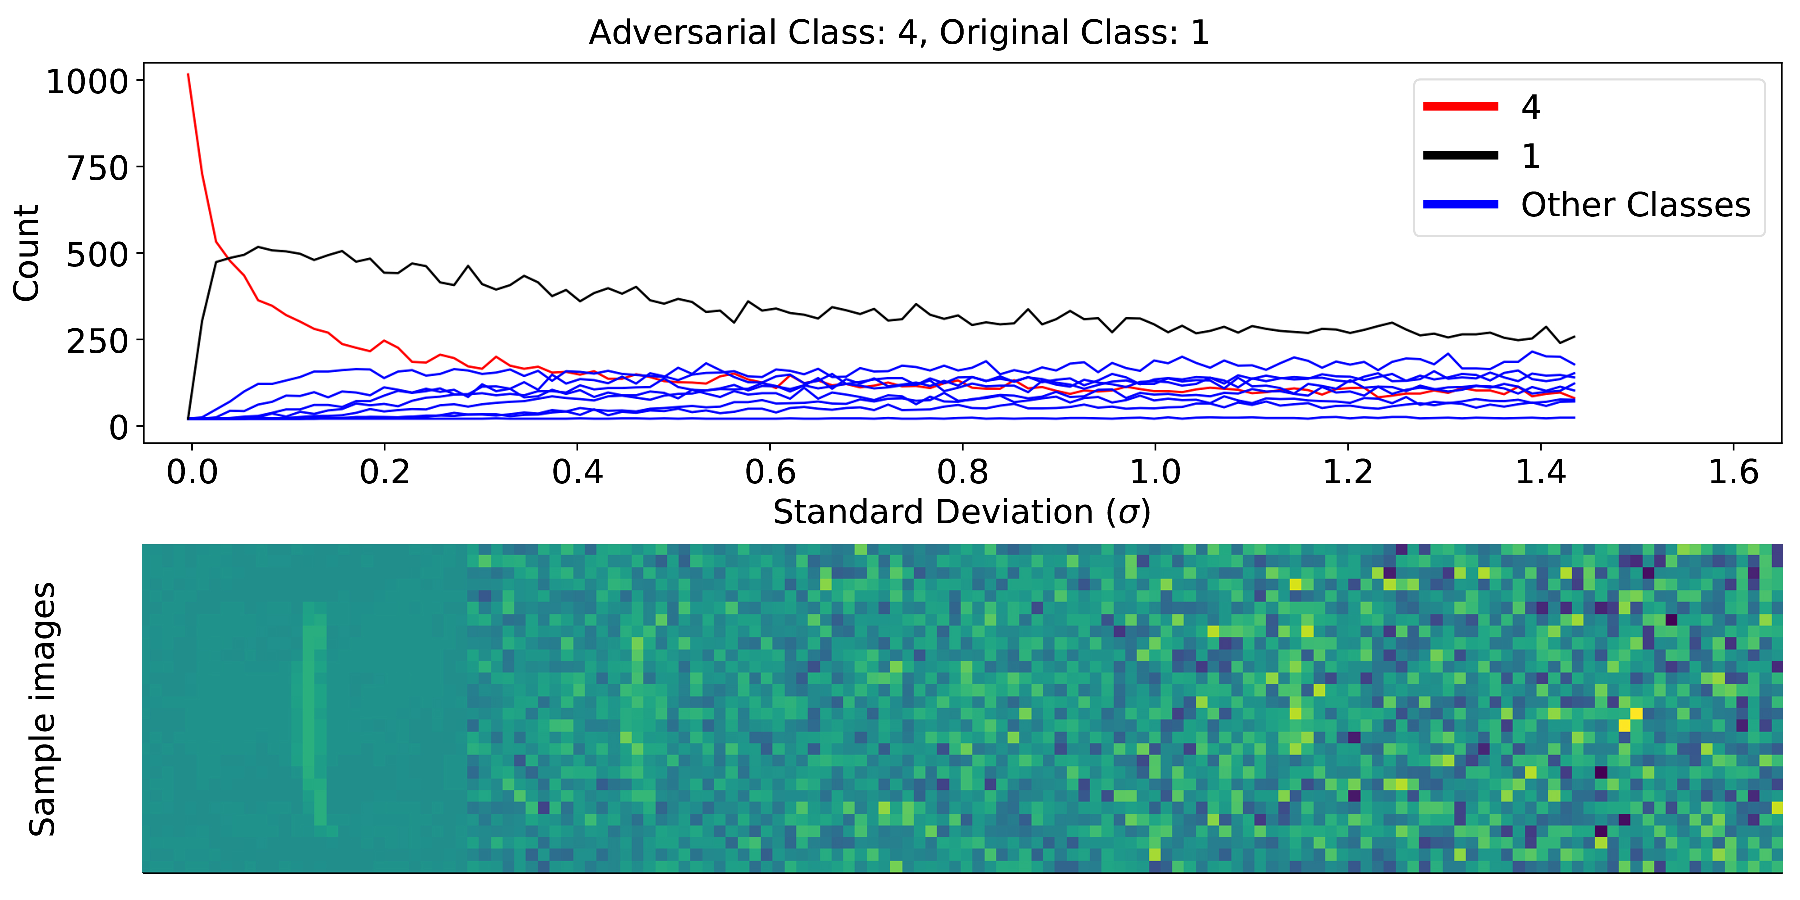
\includegraphics[width=.49\textwidth]{c2_figures/MNISTA4O1.pdf}
    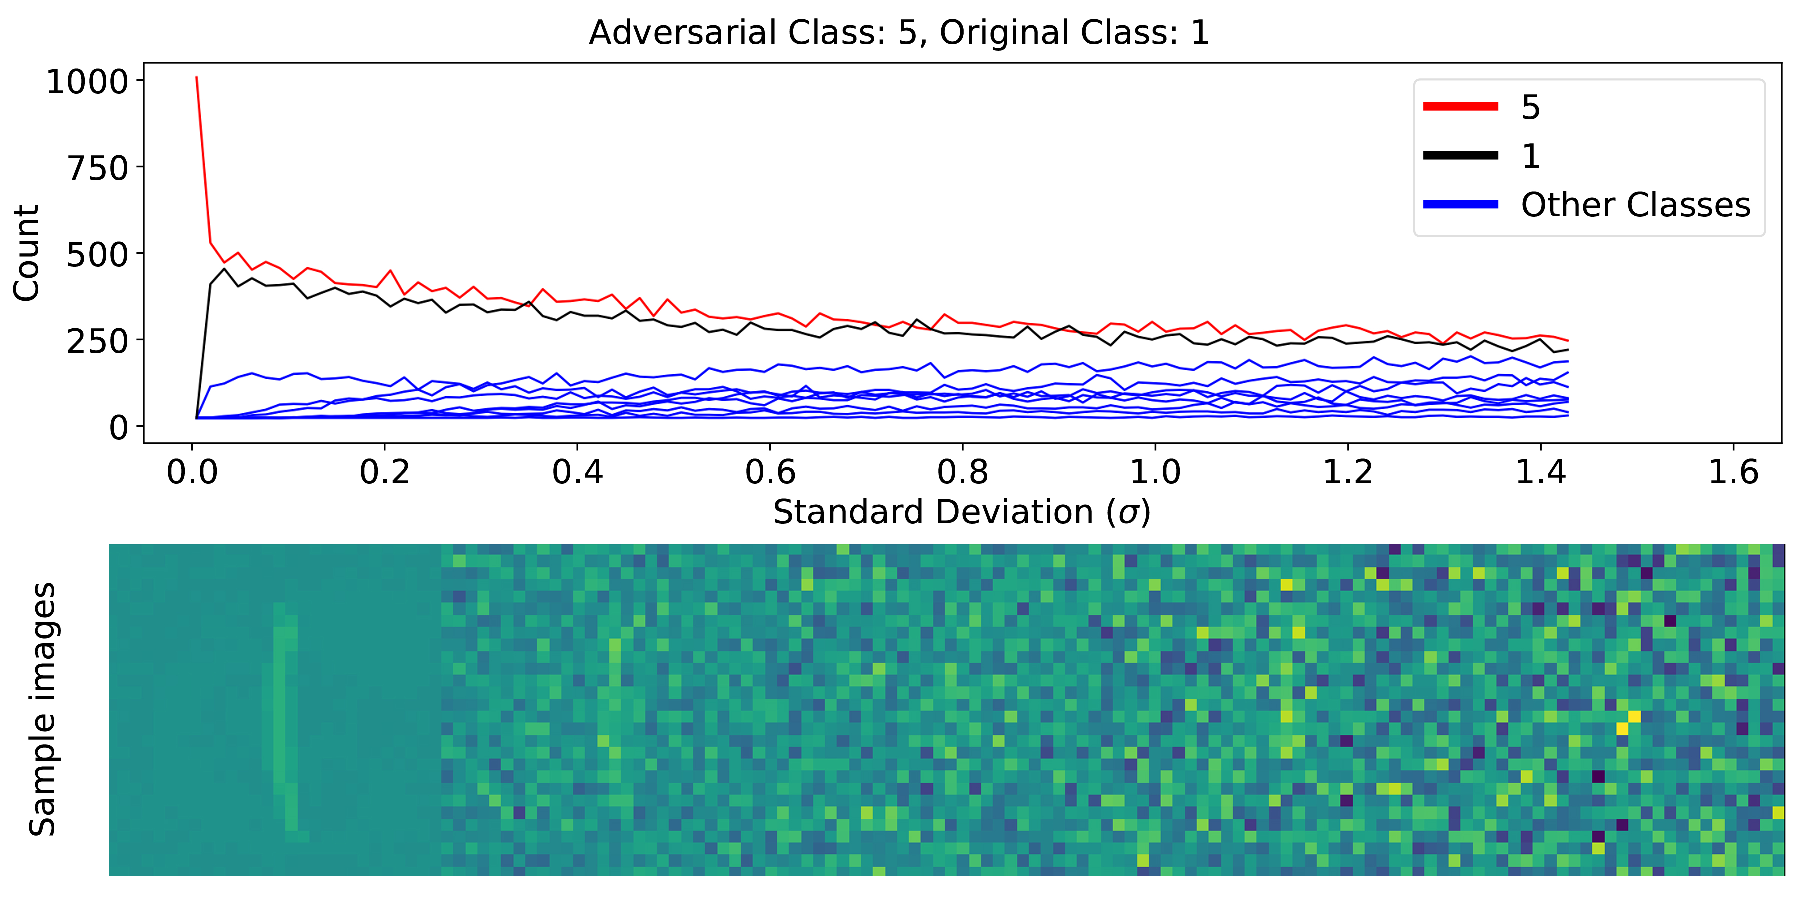
\includegraphics[width=.49\textwidth]{c2_figures/MNISTA5O1.pdf}
    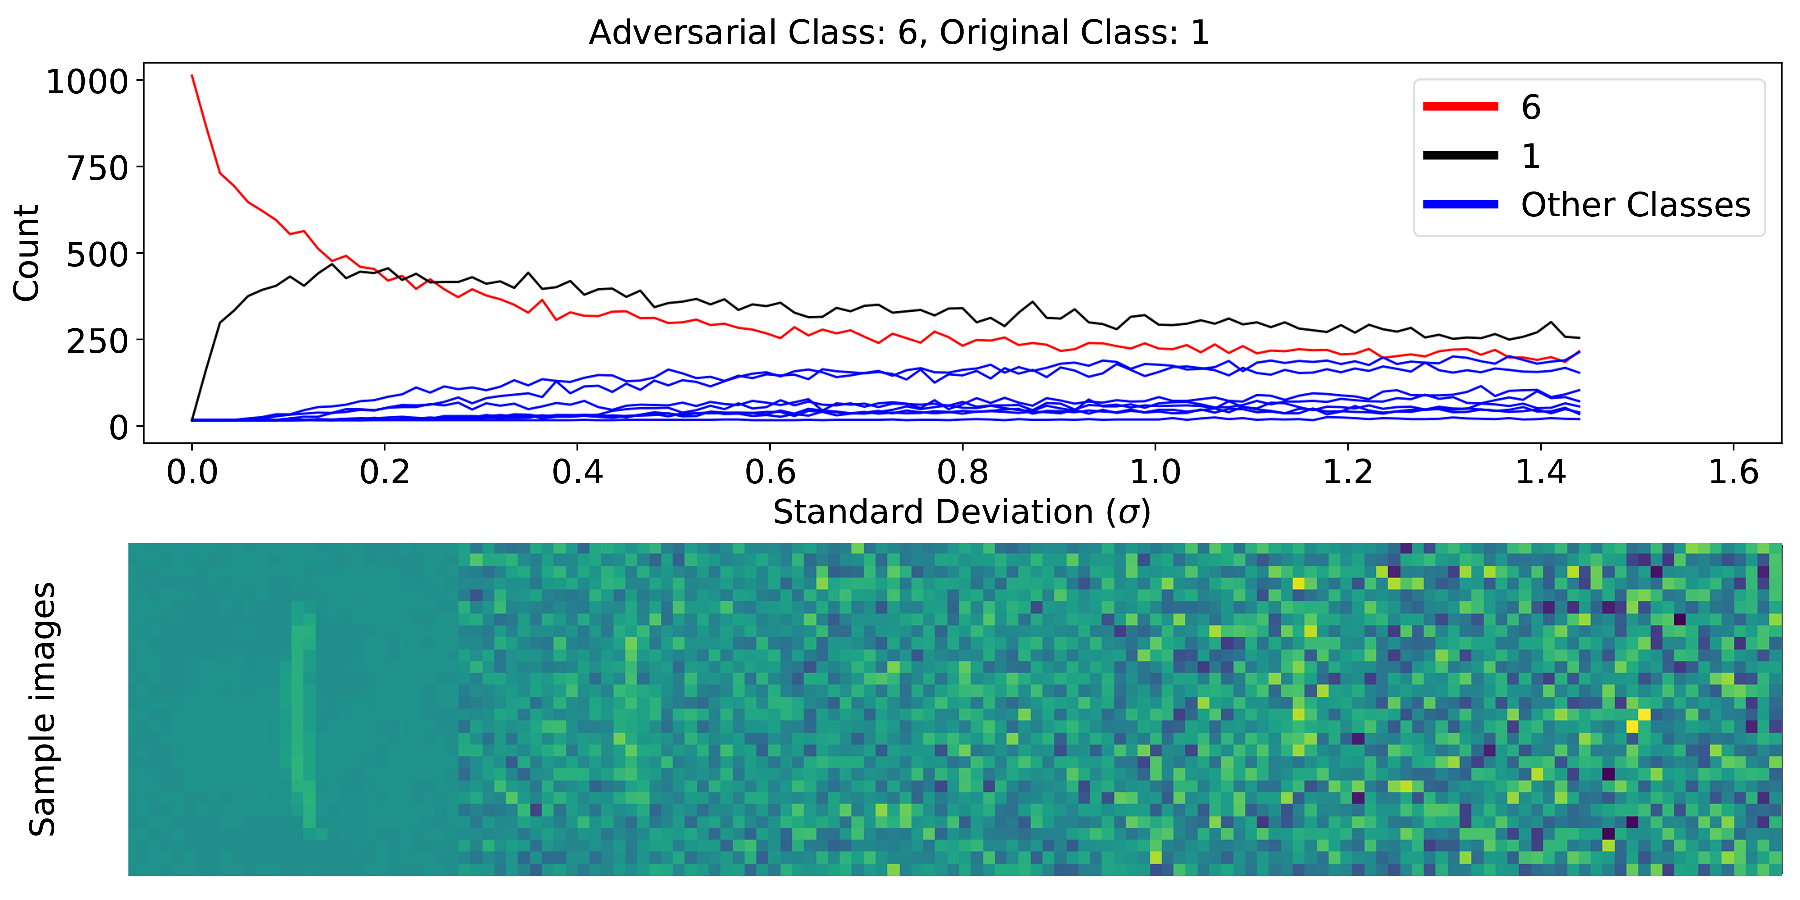
\includegraphics[width=.49\textwidth]{c2_figures/MNISTA6O1.pdf}
    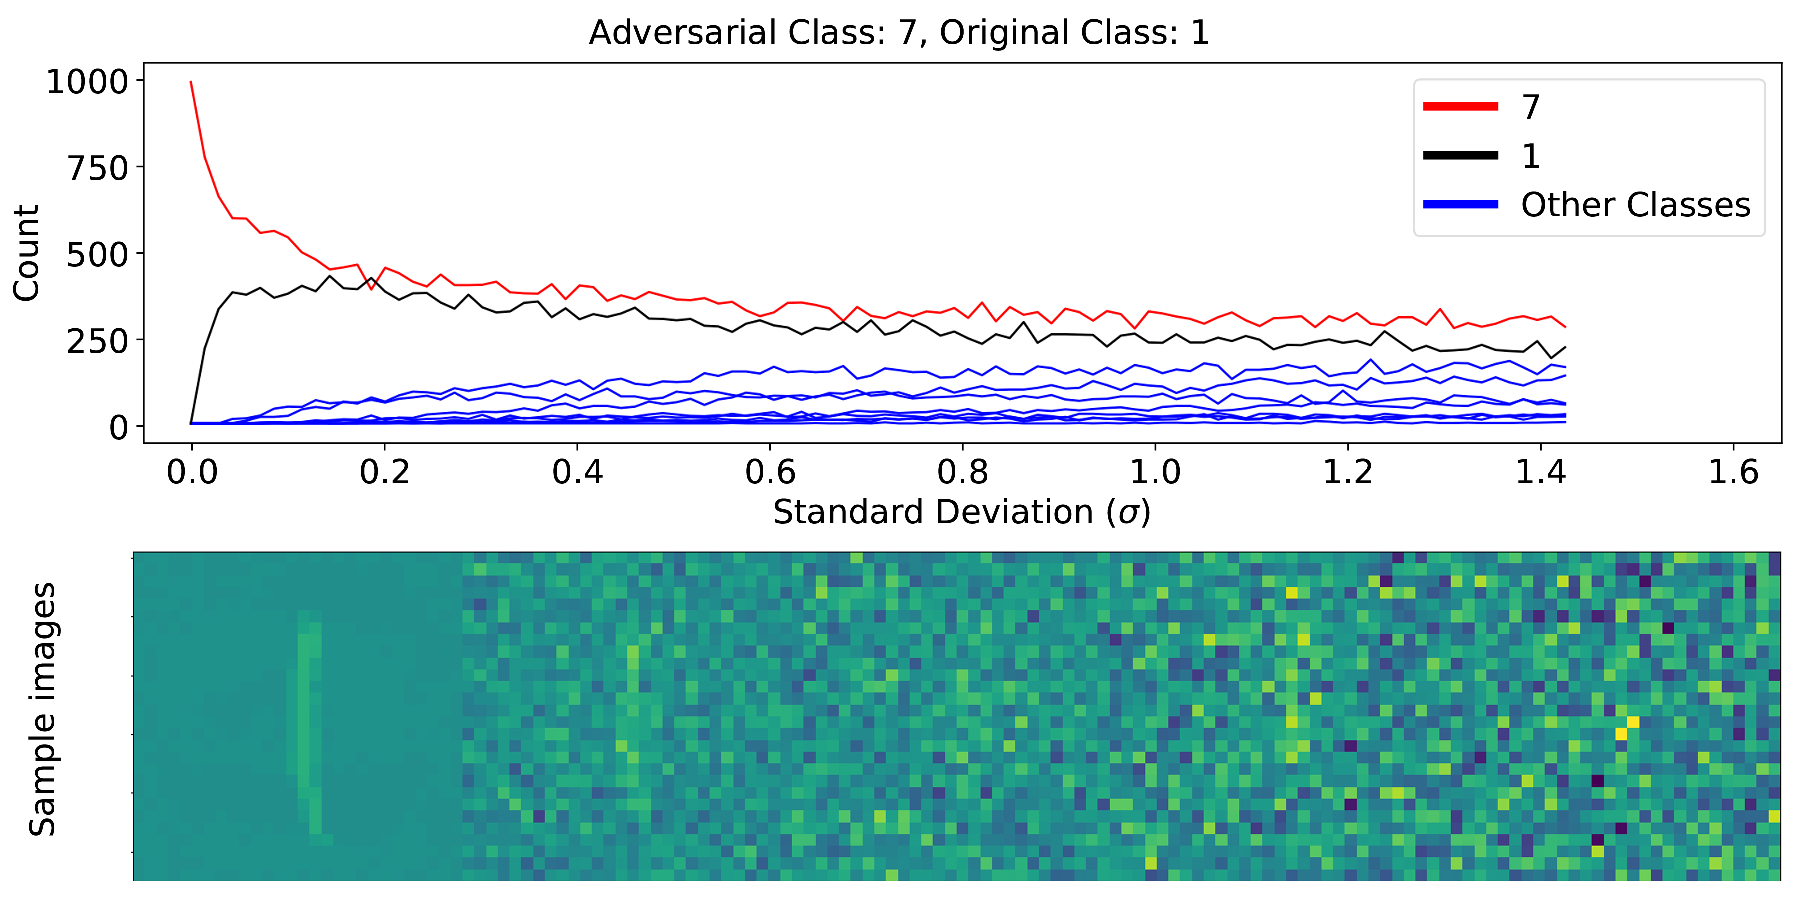
\includegraphics[width=.49\textwidth]{c2_figures/MNISTA7O1.pdf}
    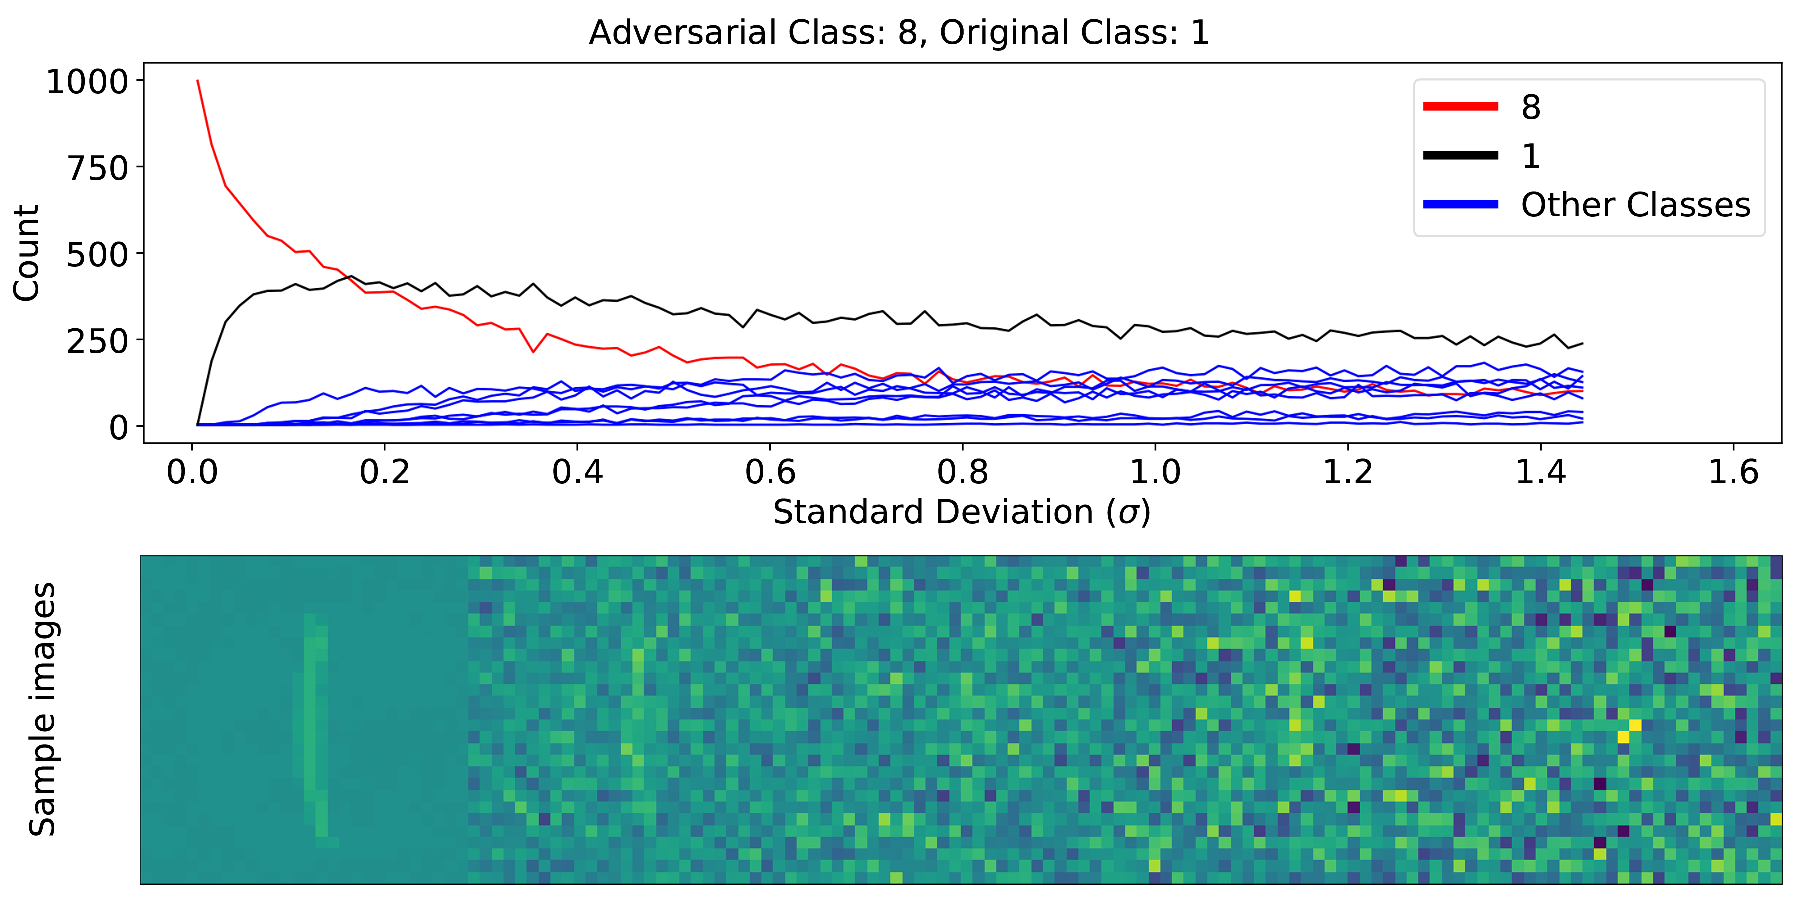
\includegraphics[width=.49\textwidth]{c2_figures/MNISTA8O1.pdf}
    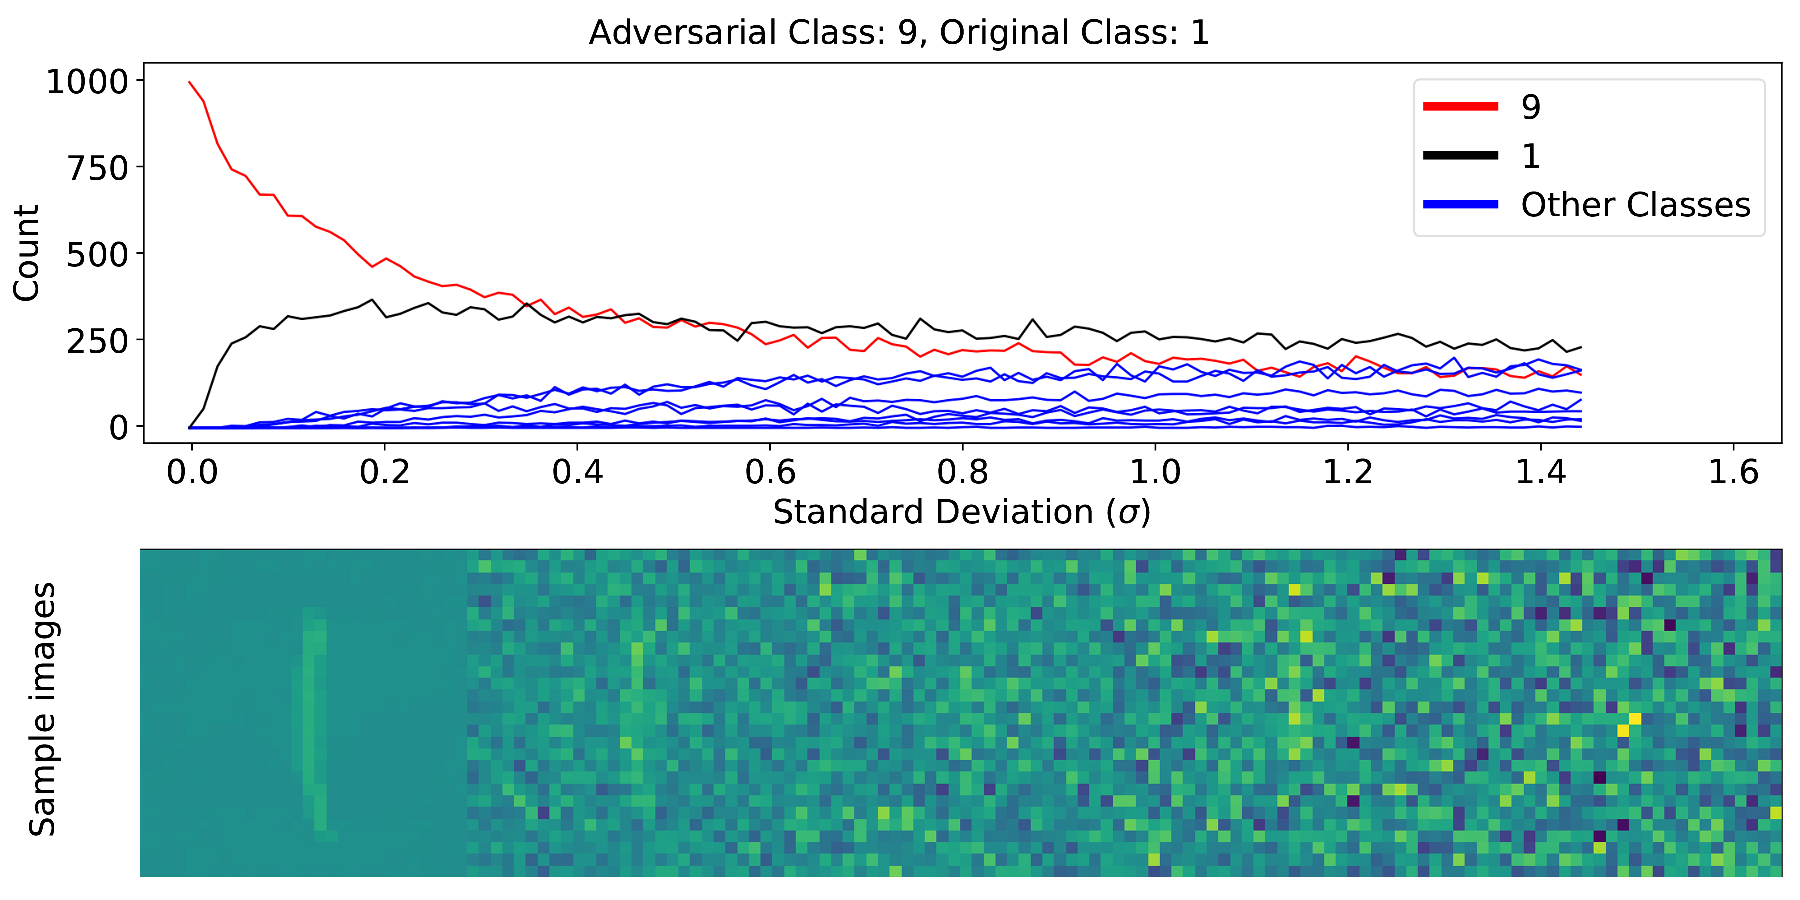
\includegraphics[width=.49\textwidth]{c2_figures/MNISTA9O1.pdf}
    \caption{Frequency of each class in Gaussian samples with increasing standard deviations around adversarial attacks of an image of a \texttt{1} targeted at classes \texttt{2} through \texttt{9} on a DNN classifier generated using IGSM. The adversarial class is shown as a red curve. The natural image class (\texttt{1}) is shown in black. Bottoms show example sample images at different standard deviations.}
    \label{fig:mnistadv}
\end{figure}

We also show histograms corresponding to those in Figure \ref{fig:IGSMpersistenceMNIST} and the networks from Table \ref{table1}.  As before, for each image, we used IGSM to generate 9 adversarial examples (one for each target class) yielding a total of 1800 adversarial examples. In addition, we randomly sampled 1800 natural MNIST images. For each of the 3600 images, we computed $0.7$-persistence. In Figure \ref{fig:FC10}, we see histograms of these persistences for the small fully connected networks with increasing levels of regularization. In each case, the test accuracy is relatively low and distortion relatively high. It should be noted that these high-distortion attacks against models with few effective parameters were inherently very stable -- resulting in most of the ``adversarial'' images in these sets having higher persistence than natural images. This suggests a lack of the sharp conical regions which appear to characterize adversarial examples generated against more complicated models.  In Figure \ref{fig:FC100200} we see the larger fully connected networks from Table \ref{table1} and in Figure \ref{fig:CNNs} we see some of the convolutional neural networks from Table \ref{table1}. 

\begin{figure}[!htb]
\centering
\includegraphics[trim=200 80 100 100, clip,width=.32\textwidth]{c2_figures/FC10-4-gamma1_hist.png}
\includegraphics[trim=200 80 100 100, clip,width=.32\textwidth]{c2_figures/FC10-2-gamma1_hist.png}
\includegraphics[trim=200 80 100 100, clip,width=.32\textwidth]{c2_figures/FC10-0-gamma1_hist.png}
\caption{Histograms of $0.7$-persistence for FC10-4 (smallest regularization, left), FC10-2 (middle), and FC10-0 (most regularization, right) from Table \ref{table1}. Natural images are in blue, and adversarial images are in red. Note that these are plotted on different scales -- higher regularization forces any "adversaries" to be very stable.\vspace{2em} }
\label{fig:FC10}
\end{figure}

\begin{figure}[!htb]
\centering
\includegraphics[trim=200 80 100 100, clip,width=.49\textwidth]{c2_figures/FC100-100-10-gamma1_hist.png}
\includegraphics[trim=200 80 100 100, clip,width=.49\textwidth]{c2_figures/FC200-200-10-gamma1_hist.png}
\caption{Histograms of $0.7$-persistence for FC100-100-10 (left) and FC200-200-10 (right) from Table \ref{table1}. Natural images are in blue, and adversarial images are in red.}
\label{fig:FC100200}
\end{figure}

\begin{figure}[!htb]
\includegraphics[width=.49\textwidth]{c2_figures/MNIST-C-4-0-stab_compare_a_var-hist.png}
\includegraphics[width=.49\textwidth]{c2_figures/MNIST-C-32-0-stab_compare_a_var-hist.png}
\includegraphics[width=.49\textwidth]{c2_figures/MNIST-C-128-0-stab_compare_a_var-hist.png}
\includegraphics[width=.49\textwidth]{c2_figures/MNIST-C-512-0-stab_compare_a_var-hist.png}
\caption{Histograms of $0.7$-persistence for C-4 (top left), C-32 (top right), C-128 (bottom left), and C-512 (bottom right) from Table \ref{table1}. Natural images are in blue and adversarial images are in red.}
\label{fig:CNNs}
\end{figure}

\subsection{Additional figures for ImageNet}

In this section we show some additional figures of Gaussian sampling for ImageNet. In Figure \ref{fig:moreimagenet} we see Gaussian sampling of an example of the class \texttt{indigo\_bunting} and the frequency samplings for adversarial attacks of \texttt{goldfinch} toward \texttt{indigo\_bunting} (classifier: alexnet, attack: PGD) and  toward  \texttt{alligator\_lizard} (classifier: vgg16, attack: PGD). Compare the middle image to Figure \ref{fig:imagenet_adv}, which is a similar adversarial attack but used the vgg16 network classifier and the BIM attack. Results are similar. Also note that in each of the cases in Figure \ref{fig:moreimagenet} the label of the original natural image never becomes the most frequent classification when sampling neighborhoods of the adversarial example. 

\begin{figure}[!htb]
    \centering
    \includegraphics[width=.32\textwidth]{c2_figures/ILSVRC2012_val_00000414-vgg16-sampling.png}
    \includegraphics[width=.32\textwidth]{c2_figures/IMNET-class-11-alexnet-PGD-48-attack_data-023.png}
    \includegraphics[width=.32\textwidth]{c2_figures/IMNET-class-11-vgg16-PGD-48-attack_data-039.png}
    \caption{Frequency of each class in Gaussian samples with increasing variance around an \texttt{indigo\_bunting} image (left), an adversarial example of the image in class \texttt{goldfinch} from Figure \ref{fig:imagenet_adv} targeted at the \texttt{indigo\_bunting} class on a alexnet network attacked with PGD (middle), and an adversarial example of the \texttt{goldfinch} image targeted at the \texttt{alligator\_lizard} class on a vgg16 network attacked with PGD (right). Bottoms show example sample images at different standard deviations.}
    \label{fig:moreimagenet}
\end{figure}


In Figure \ref{fig:persistencediffgamma}, we have plotted $\gamma$-persistence along a straight line from a natural image to an adversarial image to it with differing values of the parameter $\gamma$. The $\gamma$-persistence in each case seems to change primarily when crossing the decision boundary. Interestingly, while the choice of $\gamma$ does not make too much of a difference in the left subplot, it leads to more varying persistence values in the right subplot of Figure \ref{fig:persistencediffgamma}.  This suggests that one should be careful not to choose too small of a $\gamma$ value, and that persistence does indeed depend on the landscape of the decision boundary described by the classifier.

\clearpage
\begin{figure}[!htb]
    \centering
    \includegraphics[width=.49\textwidth]{c2_figures/persistence_interpolation-multi-sigma-IMNET-class-11-vgg16-BIM-48-attack_data-001.png}
    \includegraphics[width=.49\textwidth]{c2_figures/persistence_interpolation-multi-sigma-IMNET-class-11-vgg16-PGDL2-1008-attack_data-003.png}
%    \includegraphics[width=.32\textwidth]{persistence_interpolation-multi-sigma-IMNET-class-11-vgg16-PGDL2-1008-attack_data-005}
    \caption{The $\gamma$-persistence of images along the straight line path from an image in class \texttt{goldfinch} (11) to an adversarial image generated with BIM in the class \texttt{indigo\_bunting} (14)  (left) and to an adversarial image generated with PGL in the class \texttt{alligator\_lizard} (44) (right) on a vgg16 classifier with different values of $\gamma$. The classification of each image on the straight line is listed as a number so that it is possible to see the transition from one class to another. The vertical axis is $\gamma$-persistence and the horizontal axis is progress towards the adversarial image.}
    \label{fig:persistencediffgamma}
\end{figure}


\section{Concentration of measures} \label{sec:concentration}

We use Gaussian sampling with varying standard deviation instead of sampling the uniform distributions of balls of varying radius, denoted $U(B_r(0))$ for radius $r$ and center $0$. This is for two reasons. The first is that Gaussian sampling is relatively easy to do. The second is that the concentration phenomenon is different. This can be seen in the following proposition.

\begin{proposition} \label{prop:concentration}
    Suppose $x \sim N(0,\sigma^2 I)$ and $y \sim U(B_r(0))$ where both points come from distributions on $\RR^n$. For $\varepsilon < \sqrt{n}$ and for $\delta < r$ we find the following:
    \begin{align}
        \mathbb{P}\left[\rule{0pt}{15pt} \left| \rule{0pt}{10pt} \Norm{x} - \sigma \sqrt{n} \right| \leq \varepsilon \right] &\geq 1-2e^{-\varepsilon^2/16} \\
        \mathbb{P}\left[\rule{0pt}{15pt} \left| \rule{0pt}{10pt} \Norm{y} - r \right| \leq \delta \right] &\geq 1-e^{-\delta n/r} 
    \end{align}
\end{proposition}
\begin{proof}
    This follows from \cite[Theorems 4.7 and 3.7]{wegner2021lecture}, which are the Gaussian Annulus Theorem and the concentration of measure for the unit ball, when taking account of varying the standard deviation $\sigma$ and radius $r$, respectively.
\end{proof}

The implication is that if we fix the dimension and let $\sigma$ vary, the measures will always be concentrated near spheres of radius $\sigma \sqrt{n}$ and $r$, respectively, in a consistent way. In practice, Gaussians seem to have a bit more spread, as indicated in Figure \ref{fig:sampling}, which shows the norms of $100,000$ points sampled from dimension $n=784$ (left, the dimension of MNIST) and $5,000$ points sampled from dimension $n=196,608$ (right, the dimension of ImageNet).

\begin{figure}[htb]
    \centering
    \includegraphics[width=.5\textwidth]{./c2_figures/mnistsample.pdf}
    \includegraphics[width=.48\textwidth]{./c2_figures/imagenetsample.pdf}
    \caption{Comparison of the length of samples drawn from $U(B_7(0))$ and $N(0,7\sqrt{n})$ for $n=784$, the dimension of MNIST, (left) and $n=196,608$, the dimension of ImageNet, (right).}
    \label{fig:sampling}
\end{figure}

%Technically, it only shows one side of the bound so maybe it is not true???

%{\color{red}[K]?? So this shows that sampling via Gaussians about a data point is essentially sampling a thin annulus about the sphere of radius $\sigma\sqrt{n}$ centered at $x$.  This may mean that if we look for proportional "volume" from Gaussian sampling, we are really looking more at proportional surface area on the sphere. Could it be that this fraction is better behaved than looking at the volume fraction of the ball?  As a counterpoint though, the argument from ~\cite{inevitable2018} might indicate that it's not any better behaved.}

%{\color{blue}[DG]: I think the takeaway is that looking at balls and looking at Gaussians is almost the same as long as the radii are not too small and not too large, since in this case it affects the estimates. However, it is a one sided bound so maybe it is just affecting the estimate and not the actual behavior. It probably would be good to do some numerical experiments with Gaussians of high dimension like those in \cite[Figure 1.4]{wegner2021lecture}}

%The following is wrong. I think these two distributions are exactly the same!
%We can also look at the difference between considering perturbations of the form $y=x+ \varepsilon \triangle x$ where $\triangle x \sim N({\bf 0},1)$ and perturbations of the form $z$ where $z \sim N(x, \sigma^2 I)$. If we take $\varepsilon=\sigma$, we find that the expected length of the new vectors is the same, i.e., 
% \begin{align*}
%     \mathbb{E} [|y|] &= x+  \frac{\varepsilon}{(\sqrt{2\pi})^n}\int_{\RR^n} |y|e^{\frac{|y-x|^2}{2}}dy\\
%     &= \frac{\varepsilon}{(\sqrt{2\pi})^n}\int_{\RR^n} |w+x|e^{\frac{|w|^2}{2}}dw
% \end{align*}
% and 
% \begin{align*}
% \mathbb{E} [|z|] &= \frac{1}{(\sqrt{2\pi}\sigma)^n}\int_{\RR^n} |z|e^{\frac{|z-x|^2}{2\sigma^2}}dz \\
% &= \frac{1}{(\sqrt{2\pi})^n}\int_{\RR^n} |\sigma w+x|e^{\frac{|w|^2}{2}}dw.
% \end{align*}

% However, a similar calculation shows that 
% \[
%  \mathbb{E} \left[(|z|-\mathbb{E} [|z|])^2\right] = \sigma \mathbb{E} \left[(|y|-\mathbb{E} [|y|])^2\right]. 
% \]
% DG: I don't think I see this in the sampling...
